\documentclass[onecolumn, draftclsnofoot,10pt, compsoc]{IEEEtran}
\usepackage{graphicx}
\usepackage{url}
\usepackage{setspace}

\usepackage{geometry}
\geometry{textheight=9.5in, textwidth=7in}
\newcommand\tab[1][0.5cm]{\hspace*{#1}}


% 1. Fill in these details
\def \CapstoneTeamName{		Going Rogue Construction PROJECT MANAGEMENT APPLICATION}
\def \CapstoneTeamNumber{		37}
\def \GroupMemberOne{			Cheng Qing Lim}
\def \GroupMemberTwo{			Yuanjun Zhang}
\def \GroupMemberThree{			Dianxiong Zhang}
\def \GroupMemberFour{			Hao (Jeff) Deng}
\def \GroupMemberFive{			Robert Hudspeth}
\def \GroupMemberSix{		Shize Yuan}
\def \CapstoneProjectName{	}
\def \CapstoneSponsorCompany{	eBay, Inc}
\def \CapstoneSponsorPerson{		Luther Boorn}

% 2. Uncomment the appropriate line below so that the document type works
\def \DocType{		Winter End-Of-Term Reporting
				%Requirements Document
				%Technology Review
				%Design Document
				%Progress Report
				}
			
\newcommand{\NameSigPair}[1]{\par
\makebox[2.75in][r]{#1} \hfil 	\makebox[3.25in]{\makebox[2.25in]{\hrulefill} \hfill		\makebox[.75in]{\hrulefill}}
\par\vspace{-12pt} \textit{\tiny\noindent
\makebox[2.75in]{} \hfil		\makebox[3.25in]{\makebox[2.25in][r]{Signature} \hfill	\makebox[.75in][r]{Date}}}}
% 3. If the document is not to be signed, uncomment the RENEWcommand below
%\renewcommand{\NameSigPair}[1]{#1}

%%%%%%%%%%%%%%%%%%%%%%%%%%%%%%%%%%%%%%%
\begin{document}
\begin{titlepage}
    \pagenumbering{gobble}
    \begin{singlespace}
    	
\includegraphics[height=4cm]{coe_v_spot1}
        \hfill 
        % 4. If you have a logo, use this includegraphics command to put it on the coversheet.
        %\includegraphics[height=4cm]{CompanyLogo}   
        \par\vspace{.2in}
        \centering
        \scshape{
            \huge CS Capstone \DocType \par
            {\large\today}\par
            \vspace{.5in}
            \textbf{\Huge\CapstoneProjectName}\par
            \vfill
            {\large Prepared for}\par
            \Huge \CapstoneSponsorCompany\par
            \vspace{5pt}
            {\Large\NameSigPair{\CapstoneSponsorPerson}\par}
            {\large Prepared by }\par
            Group\CapstoneTeamNumber\par
            % 5. comment out the line below this one if you do not wish to name your team
            \CapstoneTeamName\par 
            \vspace{5pt}
            {\Large
                \NameSigPair{\GroupMemberOne}\par
                \NameSigPair{\GroupMemberTwo}\par
                \NameSigPair{\GroupMemberThree}\par
                 \NameSigPair{\GroupMemberFour}\par
                  \NameSigPair{\GroupMemberFive}\par
                   \NameSigPair{\GroupMemberSix}\par
            }
            \vspace{20pt}
        }
        \begin{abstract}
        % 6. Fill in your abstract    
       The proposed iOS project management solution for Going Rogue Design, LLC. (GRD) places an emphasis on three distinct entities: the Administrator, the Customer, and the General User. Each entity is expected to be provided with different requirements tailoring their specific needs, but the core functionality of the project would be catered towards the Customer and Administrator. The iOS application should allow Customers to obtain project information and communicate with their respective teams. Whereas the Administrator will primarily utilize a web interface that allows them to manage the details of each customer’s project. Quantitative performance metrics include load and response times under one second and server data management for twenty-five customers and fifty projects in the first roll-out. )
        \end{abstract}     
    \end{singlespace}
\end{titlepage}
\newpage
\pagenumbering{arabic}
\tableofcontents
% 7. uncomment this (if applicable). Consider adding a page break.
%\listoffigures
%\listoftables
\clearpage

% 8. now you write!
\section{Project Recap}

Going Rogue Construction project management application is a project aims to developed a software framework system to facilitate the business operation of Going Rogue Design(GRD). The project is sponsored by eBay. In addition to facilitating business operation, the team undertakes extra responsibility to ensure that the software solution not only able to facilitate the communication between the business operation and the client effectively, but also ensure to increase the efficiency of productivity within the business operation cycle.The framework of the system comprises of three separate systems, which is the web system, iOS application system, and the Firebase web services.To be more specific with the specification of web system and the iOS system, the web system is built with React, where as the iOS is built using xCode iOS 11 architecture. The architecture of the software framework system has each system serves with different purposes for our client. The iOS system serves to be an informative platform for our client, and our web system serves to be an administrative purposes website to administrate the data and the system effectively. On the other hand, the Firebase web services is a separate system serves to facilitate both the iOS system and web system, using cloud functions, Firestore database, and web hosting services. \newline


\section{Current Progress} 
 \textbf{The section below describes the current progression of the web system.}\newline

\begin{enumerate}
\item  \textbf{Login page:}\newline
The current progress of login page is completed. User should be able to access their respective accounts, and if user inputted the wrong login credential, the system will denied the access. In addition, the login system has a protected route system implemented into it which is to only allow user the access to the website content only and only when user is successfully logged in. if user is not logged in and tried to change the login URL to home URL, the system will automatically denied the access, and redirect back the web-page to the login page.\newline

 \item  \textbf{Customer Home page:}\newline
 Aside from the CSS implementation, the current progress of Customer page is completed. In this page, the Firebase database system will only allow read, write, update and delete access functionality within the Firebase collection of only "customer". For reading, the user admin should only be able to view all information about the customer user within the form of a table, where the table will display all customer related information that is stored on Firebase database. For writing, admin user should be able to create new customer account when clicking on add customer button at the bottom of the table. For deleting, the system should be able to delete the appropriate tuple/document(Firebase) of data within the Firebase database. For updating, the admin user should be able to change the value of the attribute and update the value to the Firebase database.  \newline

 \newpage
 
  \item  \textbf{Project page:}\newline
  Aside from the CSS implementation, the current progress of Project page is completed. In this page, the Firebase database system will only allow read, write, update and delete access functionality within the Firebase collection of only "Project". For reading, the user admin should only be able to view all information about the "Project" that is owned by the Customer that was clicked before the Project page. For writing, the admin user should be able to create a new project when clicking on add project button below the table. For deleting, the web system should be able to delete the appropriate tuple/document(Firebase) of data within the Firebase database. For updating, the admin user should only be able to change the value of attribute and update the value to the Firebase database except for the start date attribute. \newline 
  
\item  \textbf{Documents page:}\newline
 Include CSS and code mechanisms to support functionalities behind the scene are all finished in this page. The document page is where the App going to hook the data from firestore document collection based on the user ID and project ID where pass through the routing URL. The are three functions available in this page: add, select and delete documents. Add document will insert a document object into the database with text fields entered and an auto generated id. The select functionalities is enabled by the check box at beginning of each rows. If the check box get selected then the id of select documents are going to stored in state, if unchecked just pop off from state and the delete button will apply delete on each document ids.\newline
 
  \item  \textbf{Calendar page:}\newline
  Click the "Calendar" on the top navigation bar can give admins an accessibility to the calendar page. In the calendar page all mile stones of this project is accessible. The calendars are also listing in a table view, which shows the calendar name, calendar owner and a link to a google calendar. Click on that link it will forward to google calendar page and show details about time slots. An admin is able to add or delete calendars through provided buttons. All parts of work include CSS and functionalities are done in the calendar page.\newline
  
  \item  \textbf{Invoice page:}\newline
  All transactions and payments are able to seen at invoice page. The invoices are presenting as table rows with table headers include: invoice ID, invoice title, who made this order and the day this order placed. Except add and batch delete there has one more functionality that only invoice page have - edit. The admin is able to edit the invoice. They can edit the invoice id, invoice link, invoice name and invoice type by editing each files which separated by commas. The commas should not be deleted or added or the string tokenlizer behind the screen will failed. If user select to apply edit, then all the changes will written back to the firebase cloud. This page is completely done with CSS and React components implementation. \newline
  
  \newpage
  
  \item  \textbf{Tasks page:}\newline
  The task page is the last field which able to be accessed trough the navigation bar, all functionalities are satisfied with appropriate CSS formatting. The react hook mechanism is going to pull all tasks belong to the user and project which admin is inspecting right now. visible fields to admins are task title, task order by who, and the time it ordered. inserting and deleting functionalities are both available in this page. This page is 100 percent done.  \newline
  
  
  \item  \textbf{Edit User's Profile:}\newline
  Aside from the CSS implementation, the current progress of edit user's page is completed. In this page, the Firebase authentication system will only allow update access functionality within the Firebase services. For updating, the admin user should only be able to change the name and the photo URL (Profile picture) that the admin user wants.User email will not be allowed to be updated, due to referential integrity within the system.\newline
  
  \item \textbf{Search Engine Functionality:}\newline
  The progress of the search engine functionality is completed, except for the CSS requirement changes that is meant to increase user-friendliness for admin users. The search engine functionality uses Firebase Cloud functions to run Algolia search API, for the system to be able to search the appropriate tuple/s when searching for a specific value within the specific table/documents(Firebase) within the Firebase Firestore database. At the moment, the requirement of the search only extends to the table/document (Firebase) of "Customer", and such requirement has been fulfilled within the system. Assuming if no search result is return from the Firebase cloud function that runs the Algolia API, the table will be empty. \newline

  \item \textbf{Create admin/manager account page:}\newline
  Aside from the CSS implementation, the current progress of Create admin/manager account page is completed. In this page, the Firebase database system will only allow write access functionality within the Firebase collection of only "Customer" and "Manager". For writing, the admin user should be able to create a new admin account, and manager account that allows them to login into the web system. All functionality is successfully implemented, and no bug should ever be found in this page.\newline
  
\end{enumerate}

\begin{flushleft}
\textbf{The section below describes the current progression of the iOS system.}

\end{flushleft}

\begin{enumerate}
  \item\textbf{ Follow the Social Media:}\newline
  The iOS app is designed for two kinds of users. One type of user is the guest who doesn't have his/her own project in the company Going Rogue Design (GRD), but they are the potential customer. The other type of user is the customer who owns one or multiple projects in the company. No matter what kind of user uses the iOS app, we want to provide them the functionality to let them able to follow the Going Rogue Design (GRD) social media account such as Facebook, Instagram, etc. So that they can track the company's latest developments and events.\newline
  \item \textbf{Request Account:}\newline
  Since there are two types of users who use the iOS app, we want to make sure the guests are able to send the account request from their mobile device to the administrator. To achieve this goal, we created an open-mail functionality that will open automatically open the email app that exists in their phone and fill the content by what the guest wrote in the request form once the guest clicks the submit button in the request information form.\newline
  
  
  \item \textbf{Edit User Information}\newline
  We want users are able to check and update their personal information so that they can have better communication with the company. Also, since we want to provide our users with an easy and convenient using environment, we created the functionality of allowing users to modify their information on mobile devices. Once that information change has been submitted, we update our database immediately so that we can always save the correct latest data for the users.\newline
  \item \textbf{View and Add Contractors}\newline
  Another functionality that the iOS app provides is letting users be able to view their current contractors and give them permission to add new contractors. This feature is designed for giving the Going Rogue Design (GRD) customers a better experience in managing their project-related data because they can always view their contractors' information on their mobile device and if they have any needs, they are always being able to make a phone call to one of those contractors. About adding the contractor, once the customer submits the change, all the data will be saved to the database so that the admin knows which contractors are working with which customer.\newline
  
  \item \textbf{User Login and Unlocking Functional Tabs}\newline
  When the user first launch the app, the user will be viewing the home page by default and the user will not have the permission access to any other tabs (features) like "Projects" and "Account". The user has to log in, which will then be verified by the internal system, by proving the user is valid, and thus the other tabs (features) will be unlocked. This feature is done, however, we will need to improve the usability of this feature by implementing other functionalities to support it like a "Log Out" function for example. \newline
  
  \item \textbf{Projects Information}\newline
  This is one of the main functionality of the application as for where the verified user can view and manage one's own projects. The user can view their projects in a table list, and they can view the detail of a certain project simply by clicking it. A new view will be launched and the project detail will be displayed on top to give the user a brief overview of the project. The rest of the features, such as "documents", "tasks", "calendar", and "invoices" of the project will be available at the bottom for the user to access. This is still under development and it will be the main focus for the remaining term. \newline
  
\end{enumerate}

\newpage

\section{Left To do}

\textbf{The section below describes the current issues and bugs that are still persisting in the web system.} \newline


\begin{enumerate}
  \item \textbf{Memory Leakage} \newline
  There has a memory leak exist when the admin choose to delete a customer or a project, this happened because when delete query executed by Firestore function it will only delete the file where id matched or satisfied a query, sub-collections are not going to be deleted. In out project the admin will iterate user profiles in such order: Customer -> Projects -> project Details (tasks, invoices, documents and calendars). If any Customer or Projects get deleted the project or project detail fields are not going to be deleted, instead they are still there, this is how memory leak happened and it need to be solved.\newline
  \item \textbf{CSS for better user friendliness} \newline
  The maximum rows of a table should be defined or it will gives a bad user experience when there has thousands even hundreds of rows. Some buttons like add customer button is at bottom of a page it's not that convent to let user to scroll all the way down to the bottom of the page to find the button they want. The ideal number of line can be shown in a table should  less than a page-full volume and able to let all buttons present in the page with out using scrolling bar.\newline
  \item \textbf{A close "X" button for every Modal}\newline
  For every modal when appearing, there should be a symbol of "X" at the top right corner of the Modal, that will allow use to close the modal. Such modal can be found when clicking on "Add customer button", "delete Customer Button", "update Customer button" and so on for other tables to display the respective data. The fix should be completed before the due date.  \newline
  
     \item \textbf{Radio Button asynchronous value rendering bug}\newline
     The radio button that can be found when clicking at "add customer form", "update customer form", and so on for all form that has a radio button that only allows the user to change the value of the radio button once, or else it will not work. The particular cause of such issue is yet to be identified, but most likely happened due to the failure to assign a new value to the React system variable when the asynchronous rendering function is finished running.\newline
  
    \item \textbf{Enhance CSS to improve user friendliness}\newline
    The are several places that we can make some improvements on CSS formatting. We can rename the name of columns to let information more scent-full, for example we can change the name of "order by" to "ordered by (who)" then admin will make more sense what that column means about. The navigation bar which lead admins to traverse through the home, search, admin profiles etc, can placed at the top of the page then it will left wider space to show more details in a table. With this change we can separate the delete and edit button to different columns then user won't accidentally click on the button they intentionally don't want to click. \newline
    
\end{enumerate}

\begin{flushleft}
\textbf{The section below describes the current issues and bugs that are still persisting in the iOS system.} \newline

\begin{enumerate}
  \item \textbf{Password security and adding a log-out view}\newline 
  Currently, the login feature has several flaws that will required more development and improvements. When the user tries to enter the password in the login page, the password is not hidden hence the security is quite vulnerable. After the user logs in, though the text from the button changes to "Welcome, <first name>" from "Welcome, Sign in", there's no log out button. The logged-in user will not be able to log out but log in to other accounts. So far, the only way for the user to log out is to either clear the sign-in information in the Keychain from the Apple system, or uninstall and reinstall the app. \newline
  
  \item \textbf{The project page only display the project detail}\newline 
  The "Project" section still needs a lot of development and feature implementations. The Project page can only display a list of projects associate with the user at its current state, and the user can click on each project to view the detail of the project. The core functionalities like the documents and invoices are still needed to be implemented. This will be the goal to achieve for Spring Break and/or Spring term.\newline
  
  \item \textbf{Soft keyboard on smaller devices}\newline 
  When running the application on a smaller device like the iPhone 8, there is a small usability/user experience issue appears when a user tries to edit the account information. The "Edit Account" page has four sections where the user can modify and update it to the database. With the First and Last name text areas at the top, phone number in the middle, and address at the bottom. If the user wants to edit the phone number or address, the soft keyboard will pop up for typing, however, the keyboard blocks the editing area which disables the user to view the current editing text until the user hides the keyboard. The potential plan to resolve this issue is to push the editing areas at the top of the screen with the keyboard at the bottom, so the user can view the text while typing.\newline
\end{enumerate}

\end{flushleft}

\newpage
\section{Problems We Met During Development}

\textbf{The section below describes the hurdle faced by the iOS development team} \newline

\begin{enumerate}
  \item\textbf{Passing Data:}\newline
  One of the problems we met while developing the iOS mobile application was we don't know how to pass the data between different view controllers. The tricky part of this issue is not only because we are new to the iOS development, but it also relates with the direction we want to pass the data. In general, there are two ways to build a view controller(Screen) in Xcode, one is using the storyboard, the other is using the swift code. However, while we want to pass the data from one view controller to another, we can not do it by only using the story board. So we started to build a view controller fully programmatic to learn how to passing the data. For the data transition, there two directions. The first direction is passing the data from the current view controller to the next view controller, we know it is the 'next' view controller because we have set up the relations between them in the storyboard. To figure it out, we did some online research and we noticed we can use a function called 'prepareSegue' too solve it. The basic idea is to set up the variables in the next view controllers first for receiving the data, and in the first view controller, we used 'prepareSegue' function to get the reference of the second view controller and set up its variables data in that function. So when the screen transition happens, the data will be passed into the second view controller and the  correct data can get displayed. The second direction is passing the data in indirect way which is from the second view controller to the first view controller. To solve this problem we cannot use the 'prepareSegue' function again because the transition relation has direction. Since we have already set it up from the first view controller points to the second one, we cannot point it back from the second view controller to the first one, because it is not allowed in the Xcode. The way we solved it was using the delegate. The basic idea is to set up a protocol in the second view controller and create the needed function inside that protocol. After that, we create the delegate variable to use that protocol, so that when the event happens in the view controller, we can call the function in that delegate to solve it. Then, move back to the first view controller, we first need to set the delegate equals to it self, and then it needs to have the extension of the protocol in the second view controller. So when the function is called in the second view controller, the first view controller can have the correct reaction. These are the methods we used to pass the data back and forth between different view controllers. \newline
  
  \item\textbf{Table views and table cells:}\newline
  When developing the "Project" section of the app, we had some tedious issues with creating a table view and generating table cells for the projects. This was also due to the unfamiliarity with iOS development. We had to research and followed a few tutorials to create the table and cell views, but they were not working as expected. Most of the time that was spent with this part of the development was trying to debug the table views and cell views. After playing around with it and trying every method to narrow down the bug, we then realized that it had to do with the Storyboard's compatibility with adding features in a programmatic manner. Since this problem has been solved, each of the members learned some valuable lessons and experience for iOS development while trying to find a possible solution. \newline
  
\end{enumerate}

\begin{flushleft}
\textbf{The section below describes the hurdle faced by the web development team}

\begin{enumerate}

 \item \textbf{Unfamiliar with React JavaScript Library:}\newline
 During the early phase of the project development, the team is still yet to be very experienced with the React JavaScript library, which makes it somewhat hard for the team to work on the project. Due to the unique feature of React to somewhat enforce the style or concept of object oriented programming, together with enforcement of no functions in an object, instead of a uniquely design asynchronous function within the React system, the team has come to a learn about the many amazing things and feature about the web technology that is widely used by many people in the industry. That being said, after through multiple iteration of learning, and testing, the team now is fairly well experienced with the use of React technology and should be now very familiar with it. Each member learn to use the  React JavaScript independently, but one similarity is that we all learn as we developed, which makes is a lot more challenging and time consuming. However, it is a fun experience to be able to learn about such an amazing tool. \newline
 
 \item \textbf{Asynchronous Firebase functions: }
 One of the challenged, both the iOS and web team faced when using the Firebase library is to figure out a way to ensure that the asynchronous function has successfully completed its task, and continue on after compiling the next line of command code, when the asynchronous function is completed. Because it is asynchronous, it can be slightly challenging to figure out which particular line of code or functions requires a priority after completing the asynchronous function. Such example, can be found when rendering a table of data within the web system, when fetching a table of data from the Firebase Firestore database. Because the data retrieving function within the Firebase Firestore library is asynchronous, that has its own computer time clock at the server side, while the React who runs on the client side has its own computer time clock, the developer needs to work around with the asynchronous clock time issue. and to resolve such issue, the web team solves the problem by using React library tools called useEffect(), and useState() asynchronous function to get both clock to be synchronize to each other both at the front-end and back-end to work together that will results all system to work together. \newline
 
  \item \textbf{Appropriate use and cost efficiency of cloud function: } \newline
  Cloud function is a very interesting piece of technology that is provided by the Firebase web services, that allow us to have a server to run many functionality for our application system. Basically, you have another server that specifically take the toll on running the functionality that is needed for the entire system to work effectively, without having to risk the function to be run on the client's computer. Initially, the team tried to used cloud function to run some part of the functionality system. However, due to the lack of knowledge about server requesting, and responding functions in JavaScript and the probable expensive cost of using such technology, the technology was temporary cast at the side, while we are developing the web system. After completing the alpha stage of the system, the consideration of such powerful technology is brought up to our client, and he agreed to fund the use of such technology within our project. After many testing and time spent on development, the web team successfully built a search engine using 3rd party library provider within our Firebase cloud function. One of the struggle when using Firebase cloud function is to implement a request and responding function when receiving a return value from the Firebase cloud function server side of things. For example, if the web system sent a request to the Firebase cloud function server and which the Firebase cloud function server returns a value, the function who sent the request should also be able to respond to the server by receiving the value. It takes a lot of time and dedication to utilize the entire potential of Firebase cloud function, which the web team had done. \newline
 
 
 \item \textbf{CSS styling:}\newline
 There are several problems we met in the web part. Except the memory leak mentioned in the previous discussion. The CSS formatting on React is kind of new for all of us. We don't know why different CSS style sheets can be applied across different react components. For example a style applied on header of page A will automatically applied on another header on page B even that CSS style sheet wasn't imported in the JavaScript file of page B. This problem let us so confusing and gives a negative influence on our progress to write correct CSS formatting code.\newline  
\end{enumerate}

\end{flushleft}


\section{Description of user Study}
\textbf{The section describes the cases study and reasoning behind the design of each system. } \newline

There were no user studies conducted, but we met with senior staff at Gramor in Tualatin, Oregon to discuss the features and design traits that would best serve the project outside of the user stories that eBay Portland had created for us.
\newline \newline
\tab For the iOS app, a quick and simple interface would better serve the app so users would not be frustrated with too many menus or prompts. With only a couple of taps, and the user would be presented with exactly the information they need to complete whatever task is at hand. 
\newline \newline
\tab For the web portal, a more advanced interface is needed to serve the control that admins have over both users and projects. Minimizing screen changes and reducing adjustment time (if needed) proved to be the key traits that the interface needed. By keeping the focus on an always-familiar environment and layout, admins will never be lost when performing work. As an added bonus, when trained and accustomed to the design, they time-to-task-completion will be reduced by a substantially large factor.
\newline

\newpage

\section{Project Images}
\textbf{The section below are some of the screenshot for the web application. } \newline


\begin{enumerate}
  \item Login Page \newline\newline

\includegraphics[width=13cm, height=8cm]{web-login.png} \newline
  \item Customer (Home page)\newline\newline
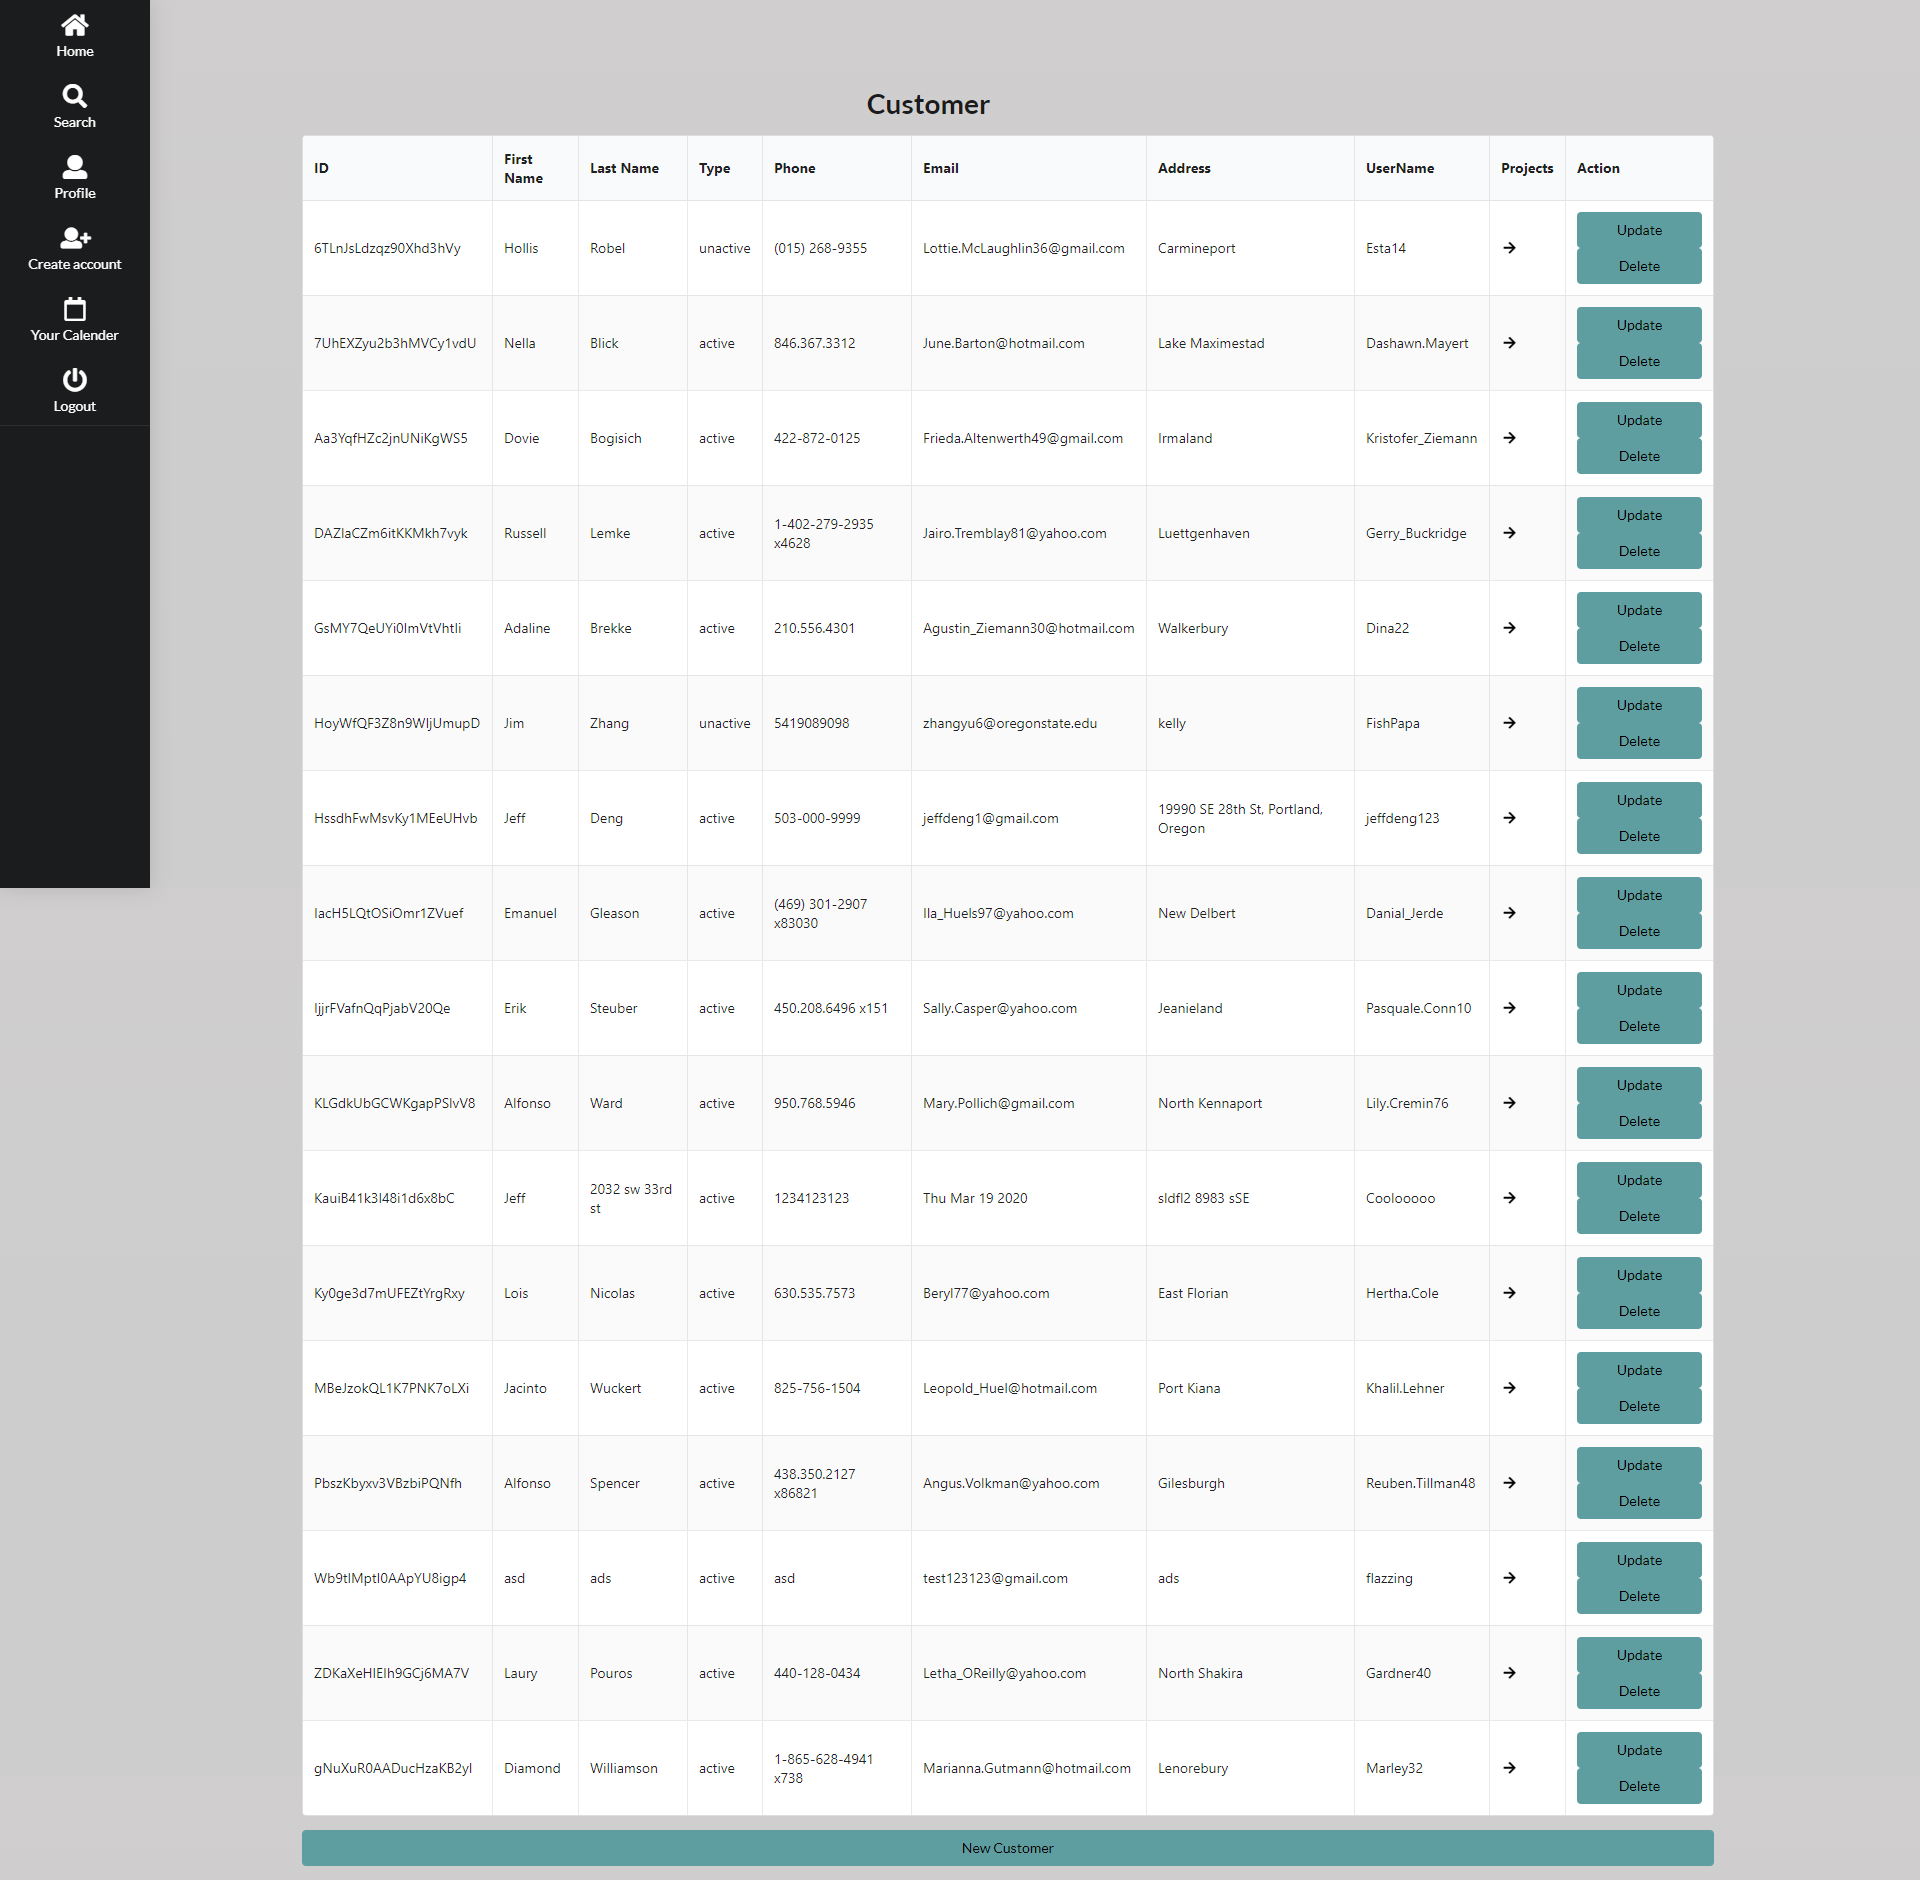
\includegraphics[width=13cm, height=8cm]{web-Customer-home.png}\newline
\newpage
    \item Project page\newline\newline
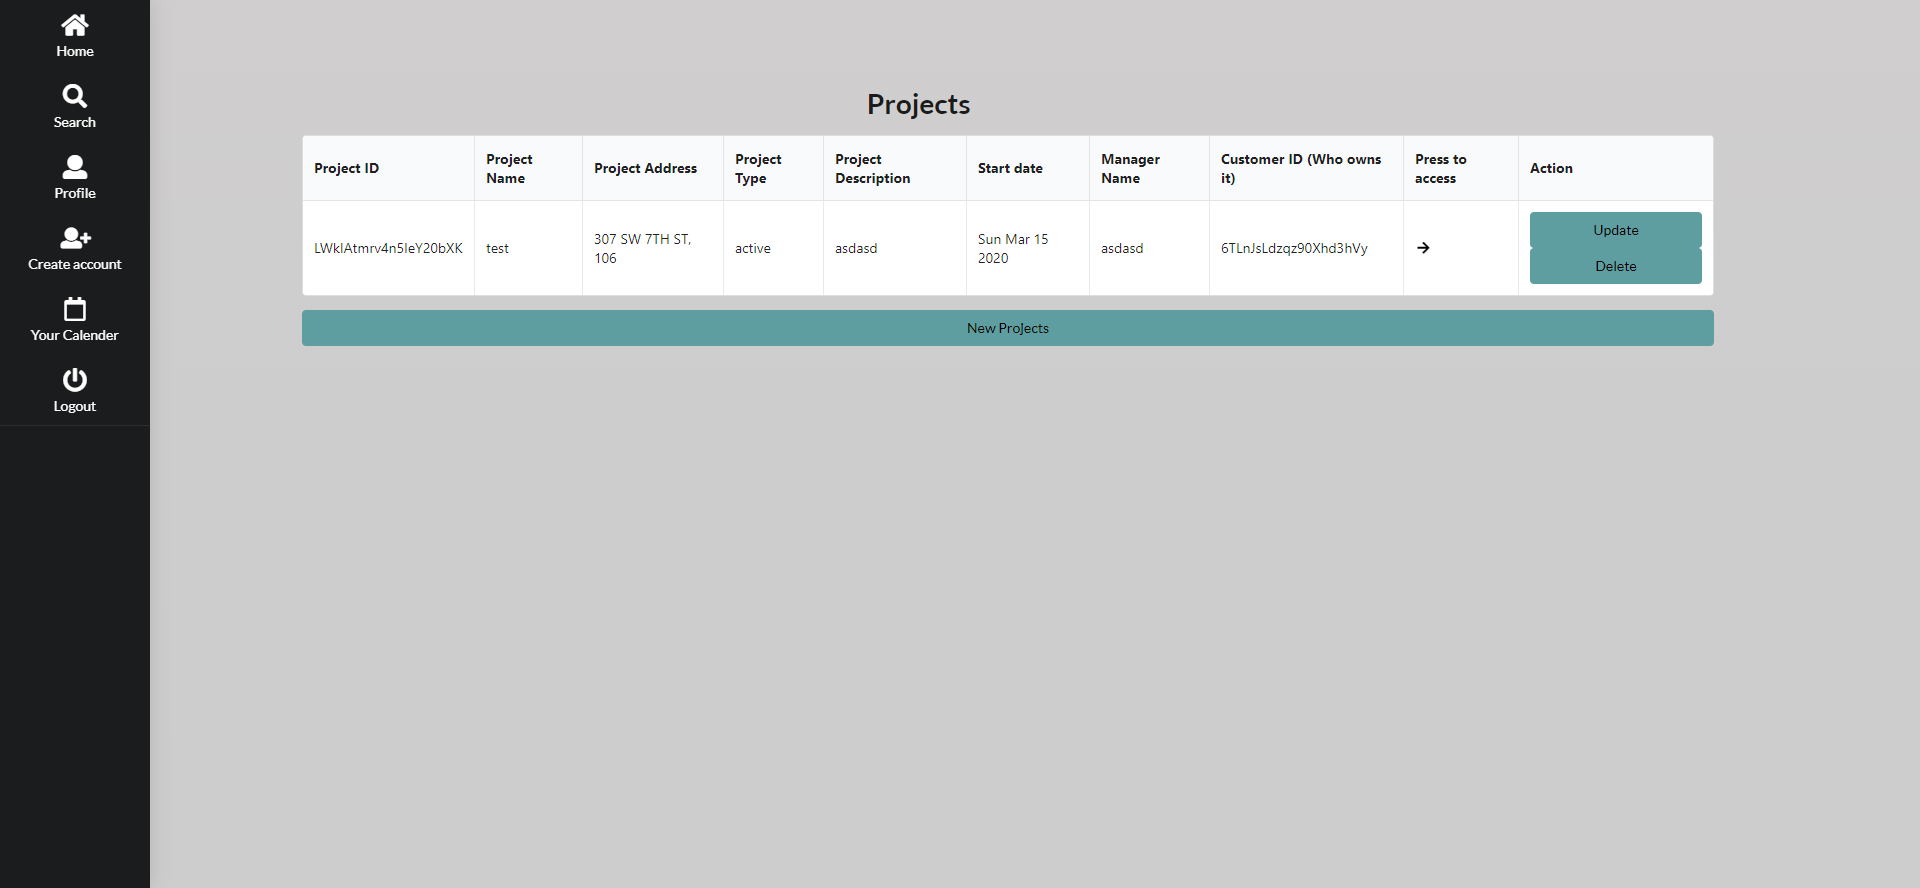
\includegraphics[width=13cm, height=8cm]{web-project.png}\newline

\item Document page\newline\newline
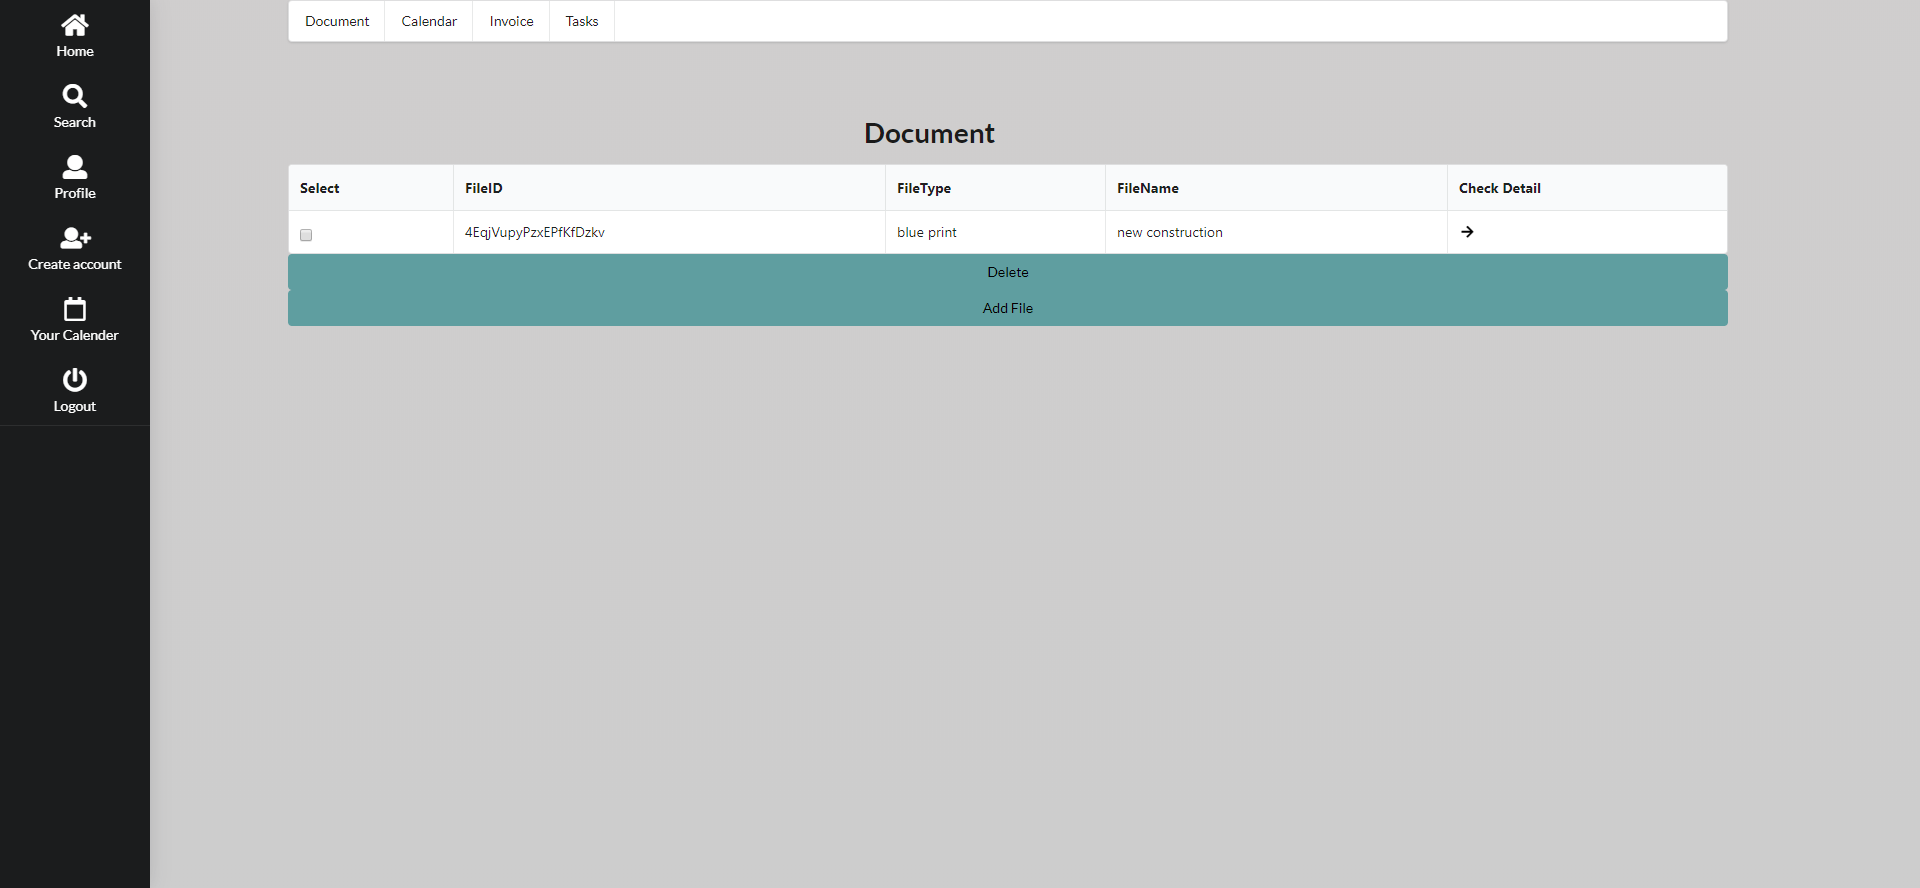
\includegraphics[width=13cm, height=8cm]{web-document-page.png}\newline
\newpage
\item Calendar page\newline\newline
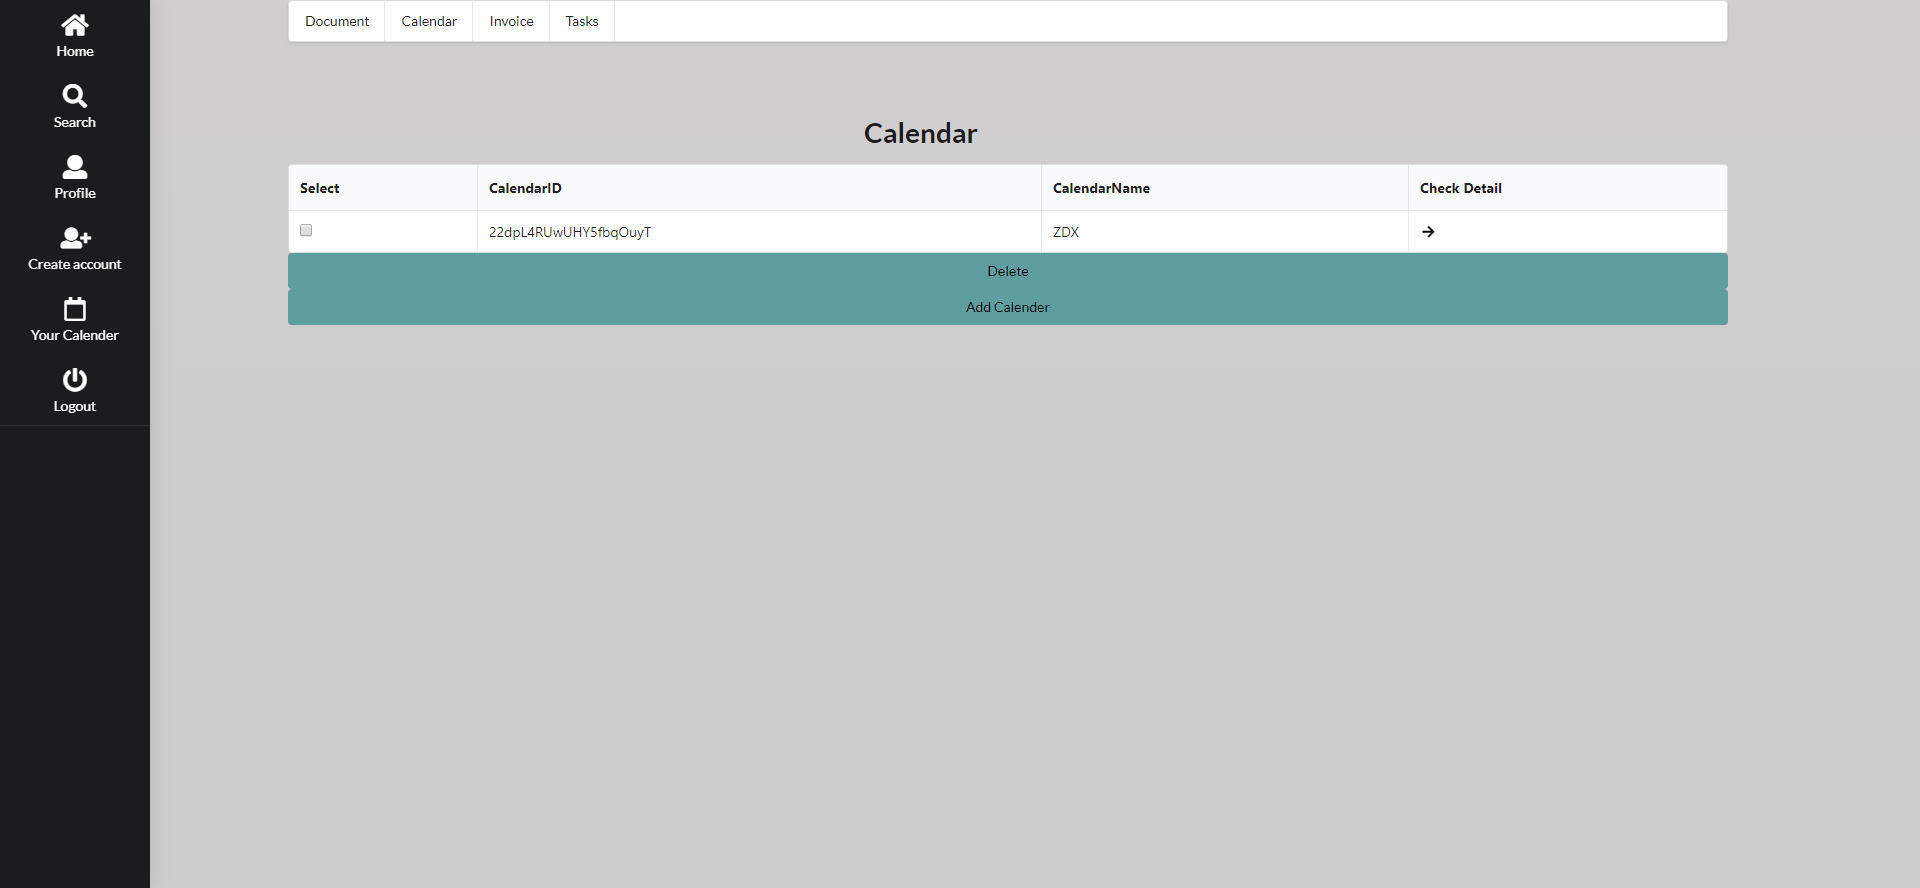
\includegraphics[width=13cm, height=8cm]{web-calendar-page.png}\newline

\item Invoice page\newline\newline
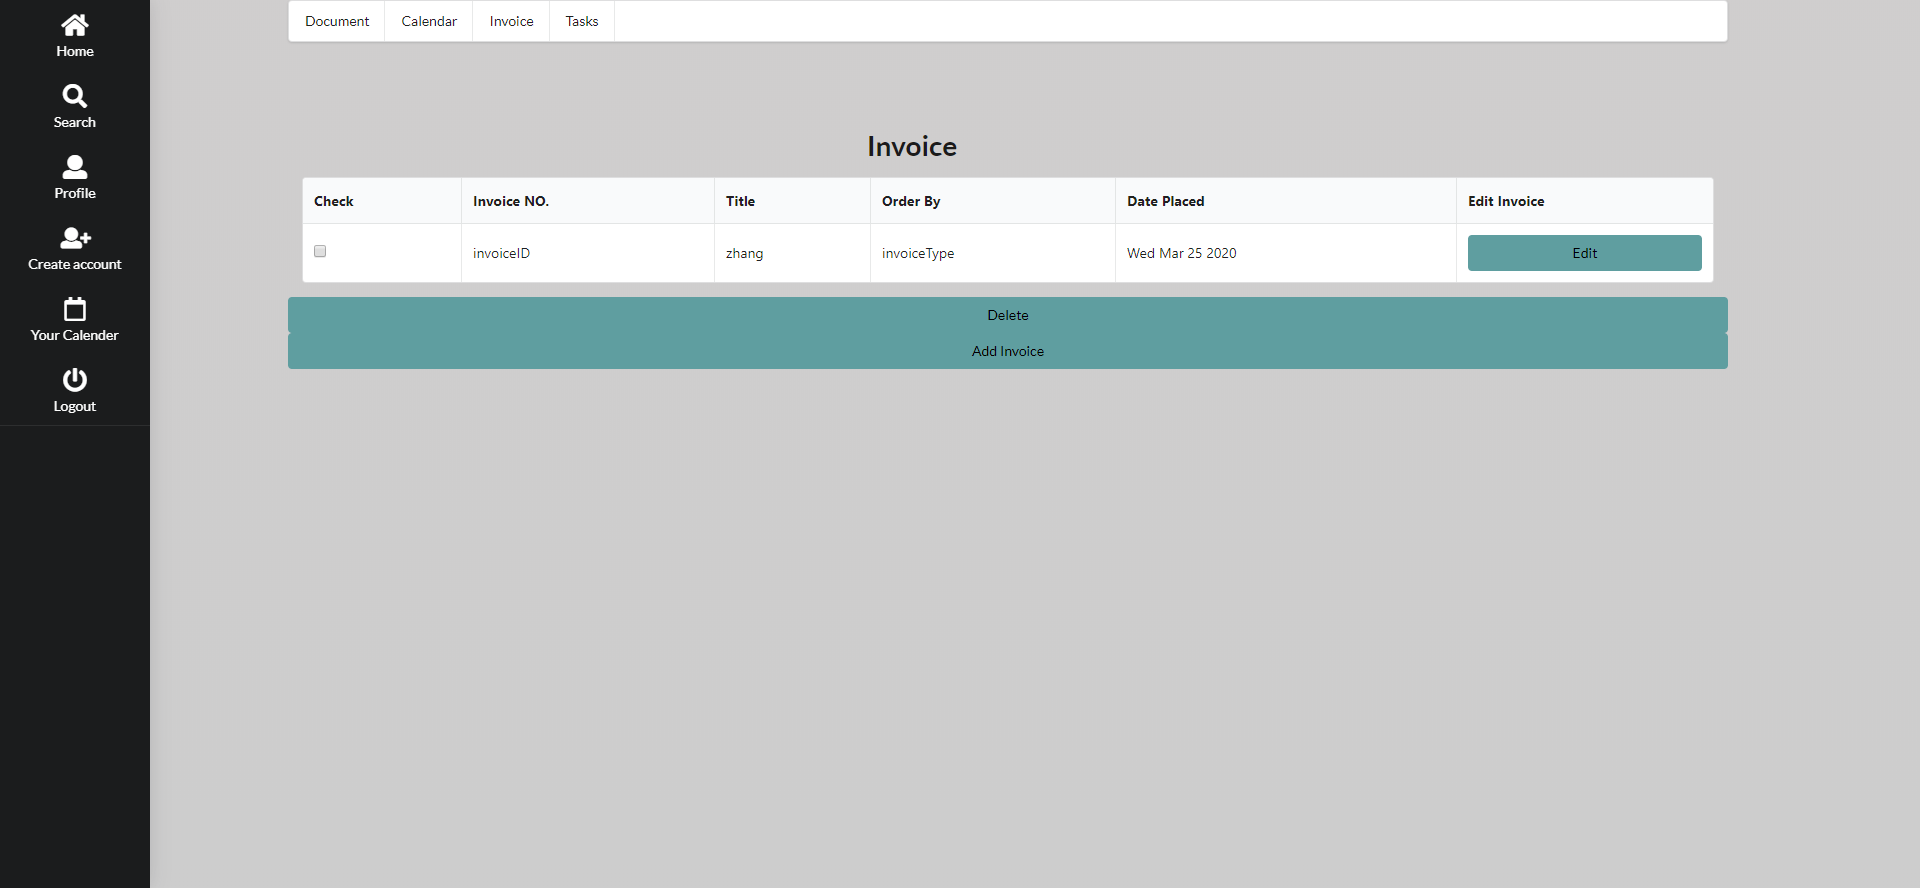
\includegraphics[width=13cm, height=8cm]{web-invoice-page.png}\newline
\newpage
\item Tasks page\newline\newline
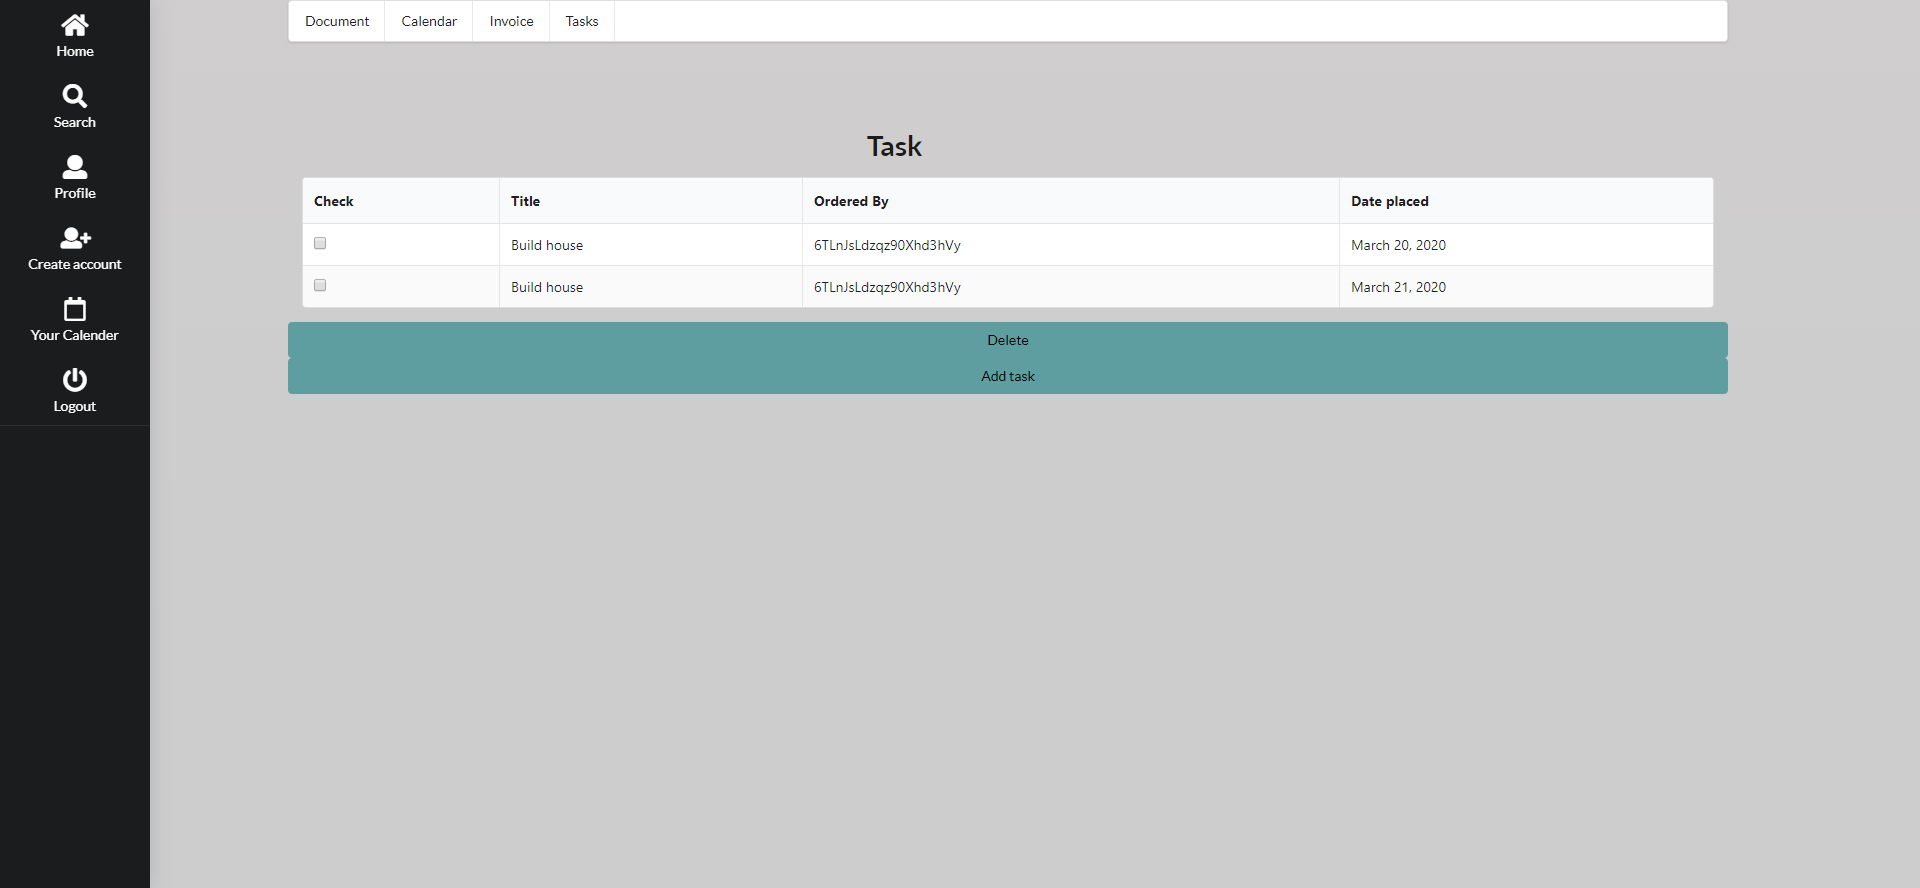
\includegraphics[width=13cm, height=8cm]{web-tasks-page.png}\newline
    
    
  \item Search page\newline\newline
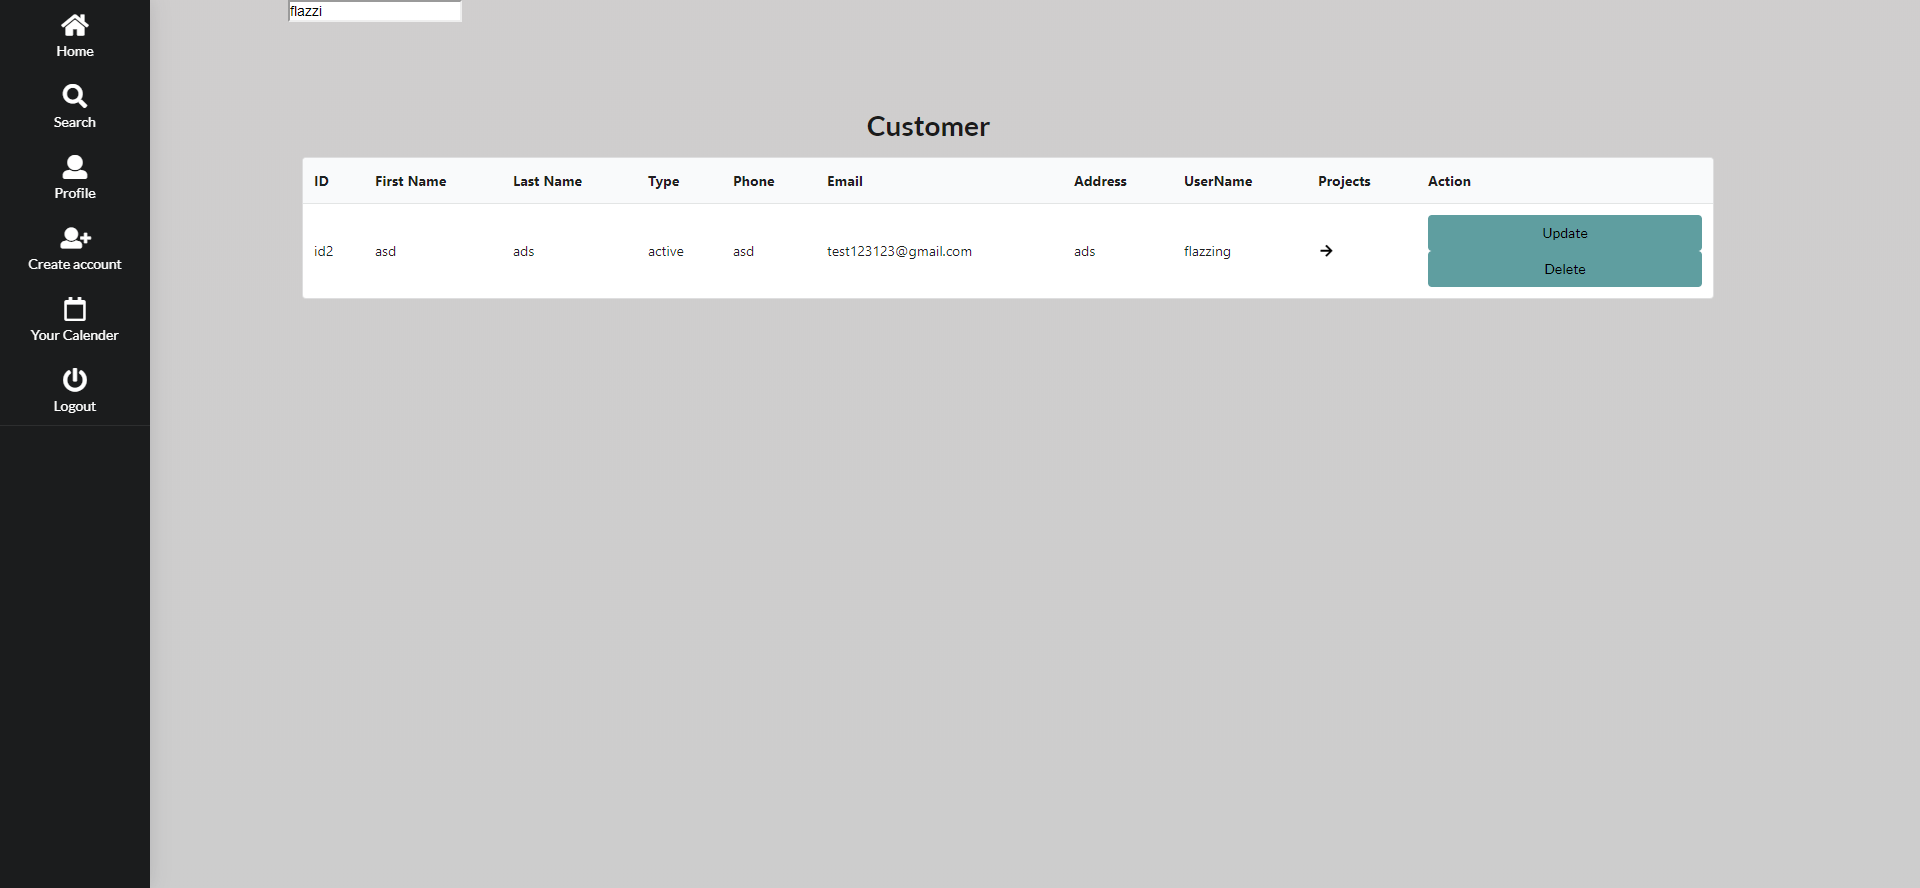
\includegraphics[width=13cm, height=8cm]{web-search-page.png}\newline
\newpage
\item Admin-profile page\newline\newline
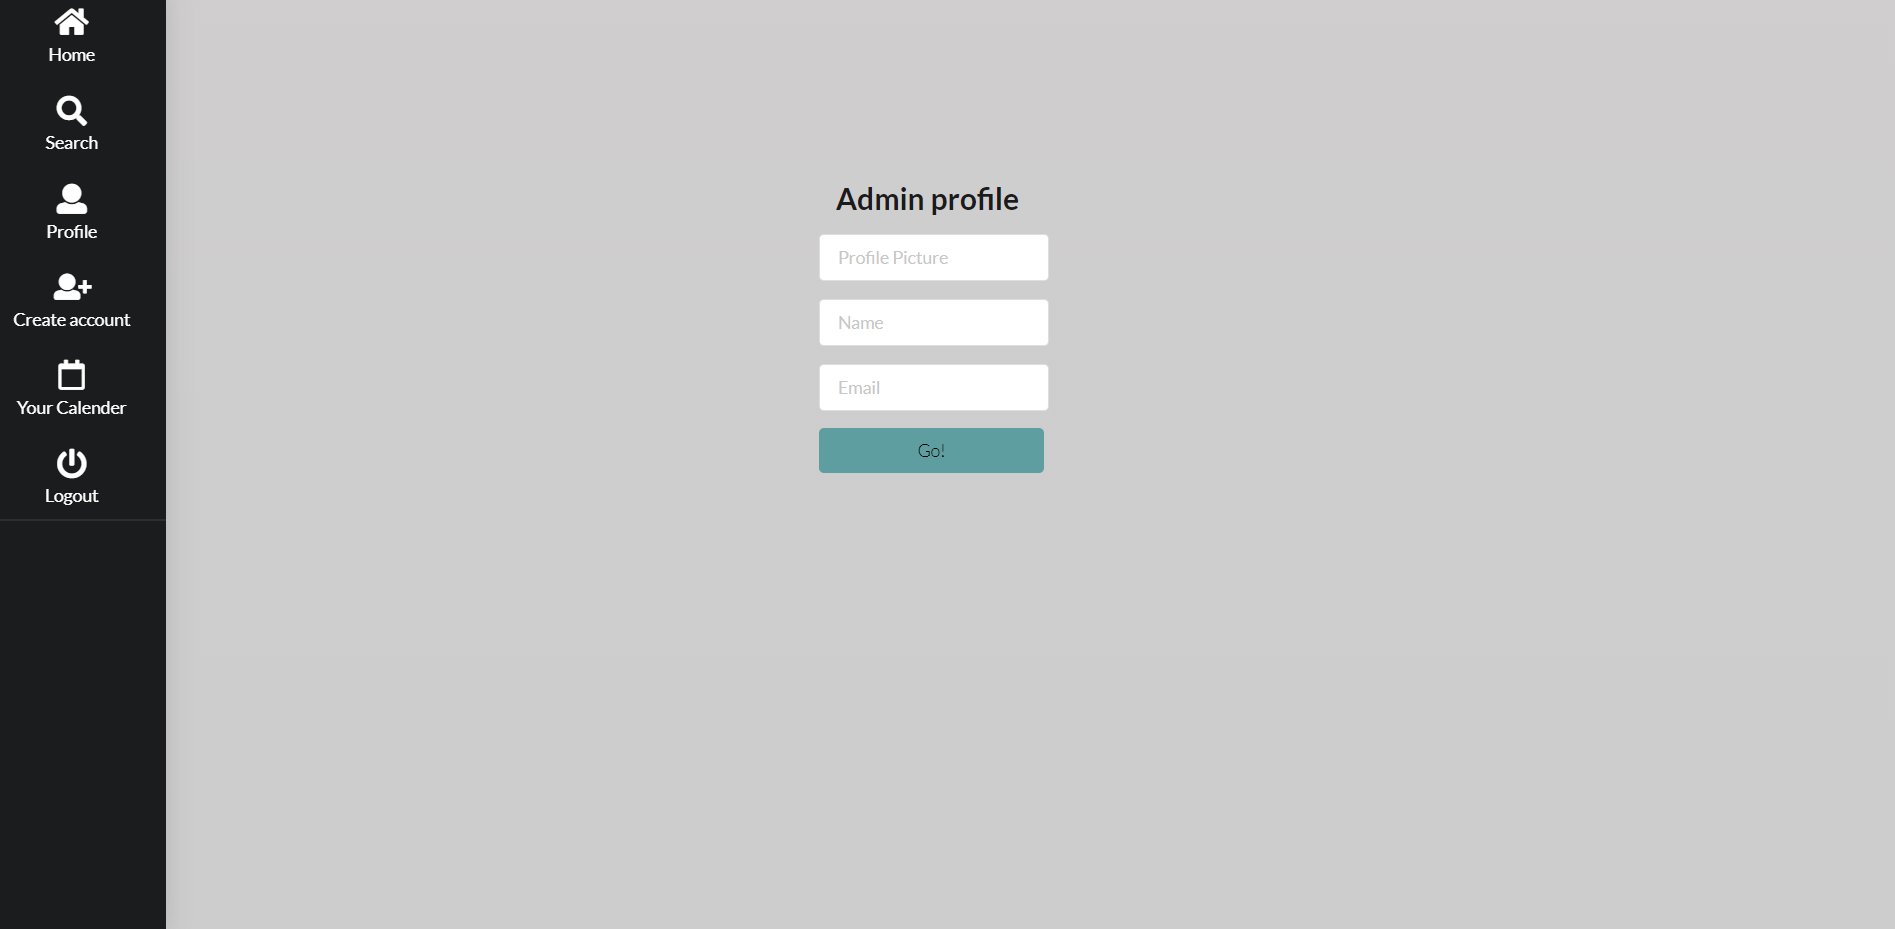
\includegraphics[width=13cm, height=8cm]{web-admin-profile-page.png}\newline
 
\end{enumerate}
\newpage
\textbf{The section below are some of the screenshot for the iOS application. } \newline

\begin{enumerate}
  \item Home Interface\newline\newline
  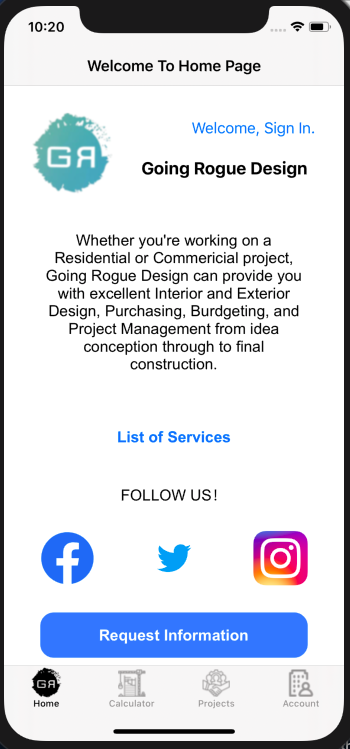
\includegraphics[width=6cm, height=13cm]{ios-home.png}\newline
  \newpage
    \item Login Interface\newline\newline
  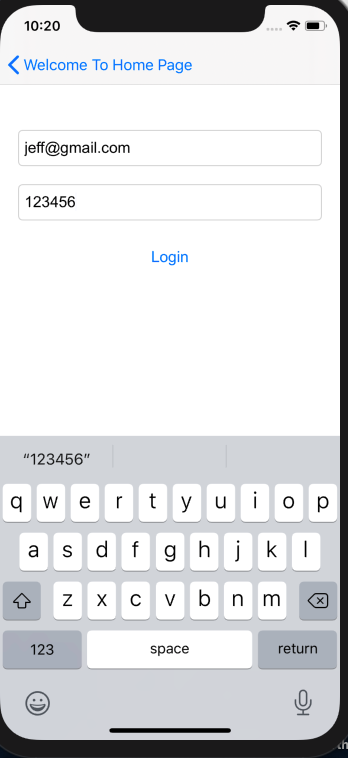
\includegraphics[width=6cm, height=13cm]{ios-login.png}\newline
  \newpage
      \item Account Interface\newline\newline
  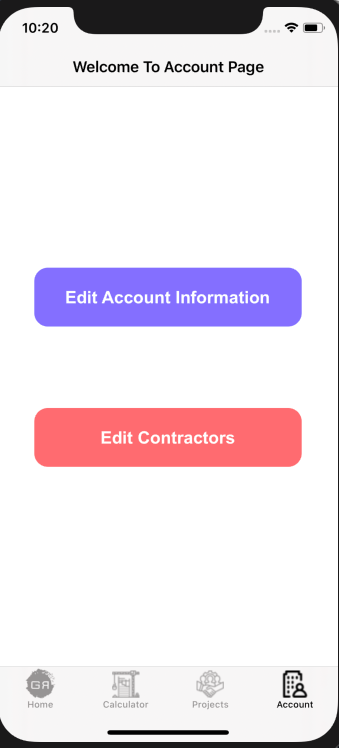
\includegraphics[width=6cm, height=13cm]{ios-account.png}\newline
  \newpage
     \item Account Edit Interface\newline\newline
  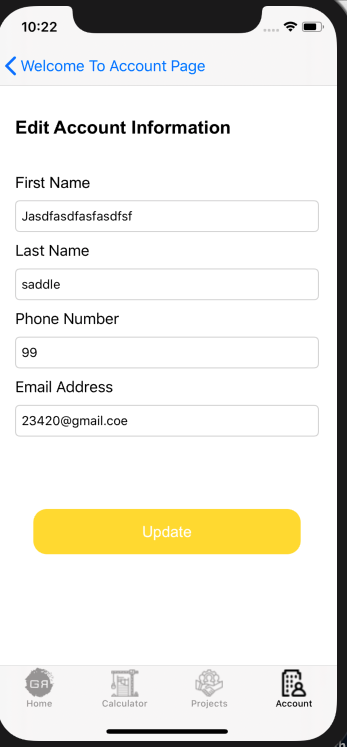
\includegraphics[width=6cm, height=13cm]{ios-edit-account.png}\newline
  \newpage
       \item Request Information Interface\newline\newline
  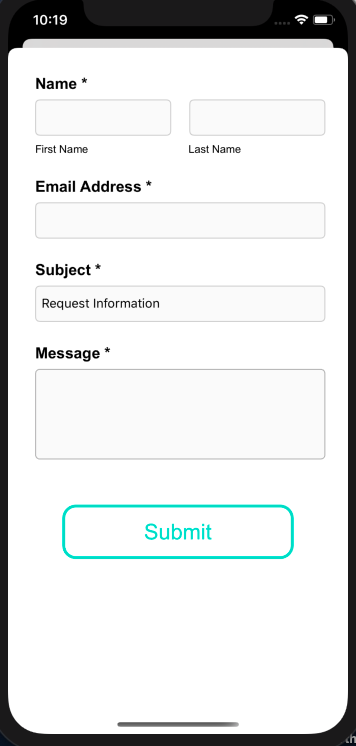
\includegraphics[width=6cm, height=13cm]{ios-request-information.png}\newline
  \newpage
  \item List of Services Interface\newline\newline
  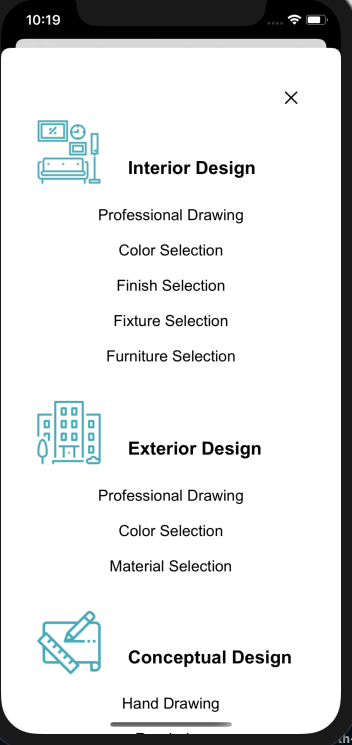
\includegraphics[width=6cm, height=13cm]{ios-list-of-services.png}\newline
  \newpage

\end{enumerate}

\end{document}